\subsection{Definition}

A slice with a hole in its centre, that means a 2D annulus, which consists of a solid of a constant temperature is exposed to a higher temperature at the surface of its hole. The aim of this calculation is to simulate the heat transfer through a homogeneous solid by the use of an axisymmetric model. Fig.~\ref{figT1} shows a sketch of the calculation area assuming a homogeneous solid, a constant temperature in the whole body at the beginning and a heating of the slice at the inner surface of the hole .

\begin{figure}[!htbp]
\centering
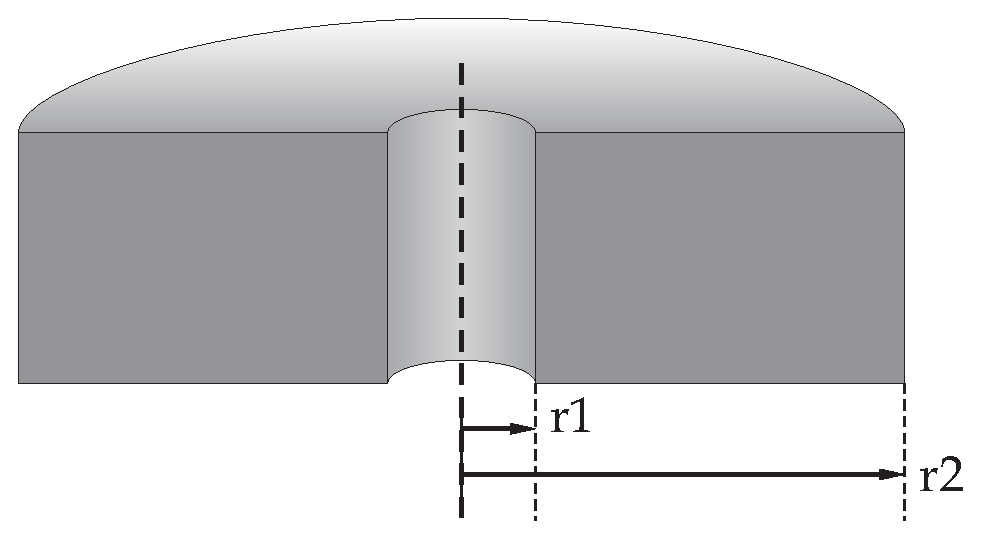
\includegraphics[width=0.5\textwidth]{PART_II/T/radial-heat-transport.eps}
\caption{\label{figT1}Radial heat conduction}
\end{figure}

%\textsl{Assumptions}
%
%\begin{tabbing}
%\=xxxxxxxxxxxxx  \=xxxxxxxxxxxxxxxxxxxxxxx \kill
%\> Temperature: \> constant temperature in the whole body at the beginning, \\
%\>  \> heating of the slice at the inner surface of the hole \\[0.5ex]
%\> Solid:		    \> homogeneous
%\end{tabbing}

The inner radius $R_1$ of the axisymmetric model is $\unit[1]{m}$ and the outer radius $R_2$ is $\unit[5]{m}$. The numerical model consists of 40 elements and 41 nodes. The initial temperature in the whole area is $\unit[25]{^{\circ}C}$. At the right boundary of the numerical model a thermal boundary condition is set with a constant value of $\unit[25]{^{\circ}C}$. At the left boundary a source term for heat flux of $q_{\mathrm{th}}=\unit[30]{W/m^2}$ is defined. Thereby the continuous heating of the solid is simulated. The used parameters of the solid are listed in Tab.~\ref{tab11}. The simulation of 5000 time steps with a constant time step length of $\unit[1000]{s}$ is done.

\begin{table}[htb]
\caption{\label{tab11}Model parameters}
\begin{center}
\begin{tabular}{llrr}
\toprule
Symbol & Parameter & Value & Unit \\
\midrule
$\rho^s$ & Density of the solid	& $\unit[2.0]{}$ & ${t \cdot m^{-3}}$ \\			
$c^s$ & Heat capacity & $\unit[900]{}$ & ${J \cdot kg^{-1} \cdot K^{-1}}$ \\
$\lambda^s$	& Thermal conductivity & $\unit[5.5]{}$ & ${W \cdot m^{-1} \cdot K^{-1}}$ \\
\hline
$q_{\mathrm{th}}$ & Heat flux & 30 & $W/m^2$ \\
$R_1,R_2$ & Inner and outer radius & 1,5 & $m$ \\
$T_0,T_2$ & Initial and boundary temperatures & 25,25 & $K$ \\
\bottomrule
\end{tabular}
\end{center}
\end{table}

\subsection{Solution}

For the heating of the annulus with the inner radius $R_1$ and the outer radius $R_2$ the following analytical solution for temperature in dependency on the radius $r$ exists.
The parameters are according to Tab. \ref{tab11}. 
%
\begin{equation}
T(r) = \frac{R_1 q}{\kappa}\ln\left(\frac{R_2}{r}\right) + T_0.
\label{T4_eq11}
\end{equation}
%
\begin{figure}[!htbp]
\centering
\includegraphics[width=0.75\textwidth]{PART_II/T/figT2.eps}
\caption{\label{figT2}Temperature distribution along the radial distance}
\end{figure}

\subsection{Results}

The results of the analytical equation for the temperature distribution over the model length are compared to those of the numerical simulation. Fig.~\ref{figT2} shows the temperature distribution over the radius of the annulus. Obviously, with the axisymmetric numerical simulation generates comprehensible results that agree well with the analytical solution.

%\clearpage

